Here we discuss the Bayesian image-deblurring experiments introduced in Section~\ref{sec:mmle_image_deblurring}. Given a blurred and noisy observation $y=Bx+\varepsilon$, obtained through an ill-conditioned blurring operator $B$ and $\varepsilon\sim\mathcal{N}(0,\sigma^2I_{d_x})$, the goal is to recover clean latent images $x$. We equip this ill-conditioned inverse problem with a total-variation prior, with strength governed by an unknown scalar parameter $\theta$. The hyper-parameter $\theta$ typically requires manual tuning but instead we estimate an optimal value by framing this as a high-dimensional \gls*{mmle} problem. With the total-variation prior, we have a non-differentiable posterior over the latent image which closely follows the setup in Section 5.3 of \citet{encinar2025proximal} and the image reconstruction problems in \citet{durmus2018efficient,goldman2022gradient}.

Let $x^\star\in\mathbb{R}^{d_x}$ denote the ground-truth image, with dimension $d_x=n_w\times n_h$. We consider  the blurring operator $B\in\mathbb{R}^{d_x\times d_x}$ following \citet{encinar2025proximal}. In particular, $B$ is a uniform local averaging operator taking the value of an interior pixel $x^\star_{ij}$ and replacing with the uniform average of a $P\times P$ neighbourhood of pixels, with truncation and renormalisation at the image boundaries. We equip the latent image $x^\star$ with the anisotropic total-variation log-prior,
\begin{equation*}
    p_\theta(x)=C(\theta)^{-1}\exp\left(-e^{\theta}\mathrm{TV}(x)\right),\qquad C(\theta)=\int_{\mathbb{R}^{d_x}}\exp\left(-e^{\theta}\mathrm{TV}(x)\right)\md x.
\end{equation*}
Positive one-homogeneity of the total-variation function and a change of variables $u=e^\theta x$ give the normalisation constant $C(\theta)\propto e^{-d_x\theta}$ which we assume to be finite for modelling purposes. The parameter $e^\theta>0$ controls the strength of this prior, which typically requires manual tuning \citep{durmus2018efficient,goldman2022gradient}. Note we exponentiate $\theta$ to ensure positivity. Here, $\mathrm{TV}(x):=\|\nabla_dx\|_1$ is the anisotropic total-variation, with $\nabla_d$ the two-dimensional discrete gradient operator, which is non-differentiable, and $\|\cdot\|_1$ is the $\ell_1$ norm. The full posterior is therefore of the form,
\begin{equation*}
    \pi_\theta(x)=p_\theta(x\mid y)\propto\exp\left(-\frac{1}{2\sigma^2}\|y-Bx\|^2_2-e^\theta\mathrm{TV}(x)-\log C(\theta)\right),
\end{equation*}
where $y$ is considered as fixed data. We may derive the gradient of the negative log-marginal likelihood using Fisher's identity,
\begin{align*}
    \nabla_\theta\ell(\theta)
    &=
    -\mathbb{E}_{x\sim \pi_\theta}
    [\nabla_\theta\log p_\theta(x,y)] .
\end{align*}
Since the log-likelihood
\begin{equation*}
    \log p(y\mid x) = -\frac{1}{2\sigma^2}\|y-Bx\|^2_2 + \text{constant}
\end{equation*}
is independent of \(\theta\), we have
\begin{equation*}
    \nabla_\theta\log p_\theta(x,y)= d_x-e^\theta\mathrm{TV}(x),
\end{equation*}
and hence
\begin{equation*}
    \nabla_\theta\ell(\theta)
    =
    \mathbb{E}_{x\sim \pi_\theta}
    [e^\theta\mathrm{TV}(x)]-d_x .
\end{equation*}
Thus the objective function is expressed as in $\eqref{eq:obj_func}$ by an expectation over $\pi_\theta$ with $F(\theta,x)=e^{\theta}\mathrm{TV}(x)-d_x$.

\subsubsection{Proximal Dynamics}

Sampling from $\pi_\theta$ for a fixed $\theta$ is challenging as the total-variation, $\mathrm{TV}(x)$, is non-differentiable. However, following \citet{encinar2025proximal}, particle algorithms applicable to the \gls*{mmle} problem may be extended to non-differentiable $p_\theta(x,y)$. In particular, letting
\begin{equation*}
    E(\theta,x):=\frac{1}{2\sigma^2}\|y-Bx\|^2+e^\theta\mathrm{TV}(x)-d_x\theta
\end{equation*}
such that $\pi_\theta(x)\propto \exp(-E(\theta,x))$, we decompose $E(\theta,x)=g_1(\theta,x)+g_2(\theta,x)$ with $g_1,g_2$ convex lower-bounded functions, $g_1$ differentiable and $g_2$ proper and lower semi-continuous. We now replace $g_2$ with the $\lambda$-\gls*{my} approximation denoted by $g_2^\lambda$ and defined,
\begin{equation*}
\begin{aligned}
    g_2^\lambda(x)&:=\min_{x'\in\mathbb{R}^{d_x}}\left\{g_2(x')+\frac{1}{2\lambda}\|x'-x\|^2\right\}\\
    &=g_2\left(\mathrm{prox}^{\lambda}_{g_2}(x)\right)+\frac{1}{2\lambda}\left\|\mathrm{prox}^{\lambda}_{g_2}(x)-x\right\|^2,
\end{aligned}
\end{equation*}
where $\mathrm{prox}^\lambda_{g_2}(x)$ is the $\lambda$-proximity mapping or proximal operator function of $g_2$ for any $\lambda>0$. We denote the full \gls*{my} approximation with $E^\lambda(\theta,x)=g_1(\theta,x)+g_2^\lambda(\theta,x)$, which is always differentiable and converges pointwise to $E(\theta,x)$ in the limit $\lambda\rightarrow0$. The gradient is given for all $x\in\mathbb{R}^d$ by
\begin{equation*}
    \nabla_xE^\lambda(\theta,x)=\nabla_x g_1(x)+\frac{1}{\lambda}(x-\mathrm{prox}^\lambda_{g_2}(\theta,x)),
\end{equation*}
where we treat $\theta$ as fixed in the minimisation over $\mathbb{R}^{d_x}$. Since $E(\theta,x)$ is continuously differentiable with respect to $\theta$, we may take $\nabla_\theta E$ gradients directly. In our setting we have $g_1=\|y-Bx\|^2_2/2\sigma^2-d_x\theta$ and $g_2=e^\theta\mathrm{TV}(x)$. Now $g_1$ is differentiable, while $g_2$ is proper and lower semi-continuous, allowing us to write the explicit gradients,
\begin{align}
    \nabla_xE^\lambda(\theta,x)&=\frac{1}{\sigma^2}B^T(Bx-y)+\frac{1}{\lambda}\left(x-\mathrm{prox}^\lambda_{e^\theta\mathrm{TV}}(\theta,x)\right),\label{eq:prox_grad_x}\\
    \nabla_\theta E(\theta,x)&=e^\theta\mathrm{TV}(x)-d_x,\label{eq:prox_grad_theta}
\end{align}
with
\begin{equation*}
    \mathrm{prox}^\lambda_{e^\theta\mathrm{TV}}(\theta,x)=\underset{x'\in\mathbb{R}^{d_x}}{\mathrm{argmin}}\left\{e^\theta\mathrm{TV}(x')+\frac{1}{2\lambda}\|x'-x\|^2\right\}.
\end{equation*}
Using these approximations and noting that for \gls*{mmle} we have $F(\theta,x)=\nabla_\theta E(\theta,x)$, we may write the proximal versions of the \gls*{pgd} particle systems with,
\begin{equation*}
    \begin{aligned}
        \md \theta_t&=-\frac{1}{N}\sum_{i=1}^N\nabla_\theta E(\theta_t,X^i_t)\md t,\\
        \md X^i_t&=-\nabla_xE^\lambda(\theta_t,X^i_t)\md t+\sqrt{2}\md B_t^i,
    \end{aligned}
\end{equation*}
which we substitute with the gradient expressions \eqref{eq:prox_grad_x}--\eqref{eq:prox_grad_theta}. We discretise the system with a Lie-Trotter splitting of the parameter and sampling dynamics, running a forward Euler step for a parameter update followed by an Euler-Maruyama step for a sampling update. This is our \gls*{mypgd} baseline as introduced in \citet{encinar2025proximal}. Similarly, we obtain the proximal version of \gls*{myholpgd},
\begin{equation*}\label{eq:high_order_langevin_scheme_proximal}
    \begin{aligned}
        \md \theta_t&=-\frac{1}{N}\sum_{i=1}^N\nabla_\theta E(\theta_t,X^i_t)\md t,\\
        \md X^i_t&=U^i_t\md t,\\
        \md U^i_t&=-\nabla_xE^\lambda(\theta_t,X^i_t)\md t+\gamma V_t^i\md t,\\
        \md V^i_t&=-\gamma U^i_t\md t-\alpha V^i_t\md t+\sqrt{2\alpha}\md B^i_t,
    \end{aligned}
\end{equation*}
where $\alpha,\gamma>0$, and Brownian motions $\{B^i\}^N_{i=1}$ are independent. We discretise the higher-order Langevin parts using the splitting scheme introduced in \citet{high_order_langevin_JMLR} and discuss a full splitting scheme discretisation in the following section. We note that we apply the \gls*{my} approximation only to the sampling dynamics, while the parameter update uses the original gradient $\nabla_\theta E(\theta,x)$. This yields the hybrid dynamics used by \citet{encinar2025proximal}. For any finite $\lambda$, the parameter update is evaluated using particles approximating the smoothed law $\pi_\theta^\lambda\propto e^{-E^\lambda(\theta,\cdot)}$, and thus incurs a small smoothing bias.

\subsubsection{\textsc{\small HOL-MYPGD} Discretisation}

We consider a Lie-Trotter splitting between the parameter updates and the sampling updates like with the \gls*{mypgd} implementation. In particular, at each iteration we sequentially step parameters using a forward Euler scheme followed by a sampling step following the discretisation scheme in \citet{high_order_langevin_JMLR}. This scheme splits the higher-order Langevin dynamics into an exactly solvable linear evolution followed by a quadrature approximation of an integrated non-linear gradient term $\nabla_x E^\lambda$. Introducing the time discretisation $0=t_0<t_1<\cdots<t_K=T$ with $t_k=kh$ and step-size $h=T/K$ we denote by $(\hat X^i_n,\hat U^i_n,\hat V^i_n)$ the discrete time approximations of $(X^i_{t_n},U^i_{t_n},V^i_{t_n})$. Then we have the Gaussian update rule,
\begin{equation*}
    \begin{aligned}
        \hat\theta_{n+1}&=\hat\theta_n-\frac{h}{N}\sum_{i=1}^N\nabla_\theta E(\hat\theta_n,\hat X^i_n),\\
        \hat X^i_{n+1}&=\hat X^i_{n}-\frac{h}{2}\Delta E^\lambda\left(\hat\theta_{n+1},\hat{X}^i_n,\hat U^i_n\right)+\mu_{12}\hat U^i_n+\mu_{13}\hat V^i_n+\xi_n^{i,1}, \\
        \hat U^i_{n+1}&=-\Delta E^\lambda\left(\hat\theta_{n+1},\hat{X}^i_n,\hat U^i_n\right)+\mu_{22}\hat U^i_n+\mu_{23}\hat V^i_n+\xi^{i,2}_n,\\
        \hat V^i_{n+1}&=\mu_{31}\Delta E^\lambda\left(\hat\theta_{n+1},\hat{X}^i_n,\hat U^i_n\right)+\mu_{32}\hat U^i_n+\mu_{33}\hat V^i_n+\xi^{i,3}_n,
    \end{aligned}
\end{equation*}
with $\xi^i_n=(\xi^{i,1}_n,\xi^{i,2}_n,\xi^{i,3}_n)\sim\mathcal{N}(0,\Sigma)$. The vector $\Delta E^\lambda(\theta,x,u)$ is chosen to be an approximation of the integral $\int_0^h\nabla_xE^{\lambda}(\theta,x+ut)dt$. We note that in \citet{high_order_langevin_JMLR}, a Lagrange interpolation is used for a high order approximation with high-order mixing guarantees; however we choose to take the simple endpoint approximation, $\Delta E^\lambda(\theta,x,u)=h\nabla_xE^\lambda(\theta,x)$ for a fair comparison against \gls*{mypgd}. We refer the reader to Section~3 of \citet{high_order_langevin_JMLR} for a more detailed review and derivation of the scheme. The constants $\mu_{12}$--$\mu_{33}$ are defined explicitly as follows,

\begin{equation*}
    \begin{alignedat}{2}
        \mu_{12}&=\left(1+\tfrac{\gamma^2}{\alpha^2}\right)h-\tfrac{\gamma^2}{2\alpha}h^2-\tfrac{\gamma^2}{\alpha^3}\left(1-e^{-\alpha h}\right),\qquad&
    \mu_{13}&=\tfrac{\gamma}{\alpha}h-\tfrac{\gamma}{\alpha^2}\left(1-e^{-\alpha h}\right),\\
    \mu_{22}&=1+\tfrac{\gamma^2}{\alpha^2}\left(1-\alpha h - e^{-\alpha h}\right),&
    \mu_{23}&=\tfrac{\gamma}{\alpha}\left(1-e^{-\alpha h}\right),\\
    \mu_{31}&=\tfrac{\gamma}{\alpha}-\tfrac{\gamma}{\alpha^2h}\left(1-e^{-\alpha h}\right),&
    \mu_{32}&=\tfrac{\gamma^3}{\alpha^2}h+\tfrac{\gamma^3}{\alpha^2}he^{-\alpha h}-\left(\tfrac{2\gamma^3}{\alpha^3}+\tfrac{\gamma}{\alpha}\right)\left(1-e^{-\alpha h}\right),\\
    \mu_{33}&=e^{-\alpha h}\left(1+\tfrac{\gamma^2}{\alpha}h\right)-\tfrac{\gamma^2}{\alpha^2}\left(1-e^{-\alpha h}\right),
    \end{alignedat}
\end{equation*}
and $\Sigma=\begin{pmatrix}
    \sigma_{11}I_{d_x} & \sigma_{12}I_{d_x} & \sigma_{13}I_{d_x} \\
    \sigma_{12}I_{d_x} & \sigma_{22}I_{d_x} & \sigma_{23}I_{d_x} \\
    \sigma_{13}I_{d_x} & \sigma_{23}I_{d_x} & \sigma_{33}I_{d_x}
\end{pmatrix}$ with,

\begin{align*}
    \sigma_{11}&=\tfrac{2\gamma^2}{\alpha^3}h-\tfrac{2\gamma^2}{\alpha^2}h^2+\tfrac{2\gamma^2}{3\alpha}h^3-\tfrac{4\gamma^2}{\alpha^3}he^{-\alpha h}+\tfrac{\gamma^2}{\alpha^4}\left(1-e^{-2\alpha h}\right),\\
    \sigma_{12}&=\tfrac{\gamma^2}{\alpha^3}\left(\alpha h - 1 + e^{-\alpha h}\right)^2,\\
    \sigma_{13}&=-\tfrac{\gamma^3}{\alpha^2}h^2\left(2e^{-\alpha h}+1\right)+\left(\tfrac{2\gamma^3}{\alpha^3}-\tfrac{\gamma^3}{\alpha^3}e^{-2\alpha h}-\tfrac{4\gamma^3}{\alpha^3}e^{-\alpha h}-\tfrac{2\gamma}{\alpha}e^{-\alpha h}\right)h+\left(\tfrac{3\gamma^3}{2\alpha^4}+\tfrac{\gamma}{\alpha^2}\right)\left(1-e^{-2\alpha h}\right),\\
    \sigma_{22}&=\tfrac{2\gamma^2}{\alpha}h-\tfrac{4\gamma^2}{\alpha^2}\left(1-e^{-\alpha h}\right)+\tfrac{\gamma^2}{\alpha^2}\left(1-e^{-2\alpha h}\right),\\
    \sigma_{23}&=\tfrac{\gamma^3}{\alpha^2}\left(e^{-2\alpha h}-2e^{-\alpha h}-2\right)h+\tfrac{3\gamma^3}{2\alpha^3}\left(e^{-2\alpha h}-4e^{-\alpha h}+3\right)+\tfrac{\gamma}{\alpha}\left(1-e^{-\alpha h}\right)^2,\\
    \sigma_{33}&=-\tfrac{\gamma^4}{\alpha^2}h^2e^{-2\alpha h}+\left(-\tfrac{2\gamma^2}{\alpha}e^{-2\alpha h}+\tfrac{\gamma^4}{\alpha^3}\left(-3e^{-2\alpha h}+4e^{-\alpha h}+2\right)\right)h\\
    &\qquad +\tfrac{\gamma^4}{2\alpha^4}\left(-5e^{-2\alpha h}+16 e^{-\alpha h}-11\right)+\tfrac{\gamma^2}{\alpha^2}\left(-3e^{-2\alpha h}+4e^{-\alpha h}-1\right)+1-e^{-2\alpha h}.
\end{align*}

\subsubsection{Image Deblurring Experimental Details}

We present two distinct blurring setups A and B with different blur and noise severity. Setup A is a severe blurring with patch size $P=10$ and added noise $\sigma=1.0$, whereas setup B is a less severe blurring with patch size $P=8$ and $\sigma=0.8$. We apply the problem to a variety of black and white images of varying sizes, which we scale to approximately the same dimension $d_x$.

Across all setups we set $N=20$ particles with independent initial states
\begin{equation*}
    X^i_0\overset{i.i.d}{\sim}\mathcal{N}(50\mathbf{1}_{d_x},30^2I_{d_x}),\qquad i=1,\ldots,N,
\end{equation*}
where each component is drawn from a Gaussian distribution with mean $50$ and standard deviation $30$ and set $\theta_0=-15$. We set the Moreau-envelope parameter $\lambda=0.4$ and run $K=6000$ iterations with a shared step-size $h=0.04$, noting that in implementation we normalise $\theta$ per pixel by the dimension $d_x$ and use the following gradient,
\begin{equation*}
    \nabla_\theta\ell(\theta)
    =
    \mathbb{E}_{x\sim \pi_\theta}
    \left[\frac{e^\theta}{d_x}\mathrm{TV}(x)-1\right].
\end{equation*}
We evaluate the proximal map using a Douglas-Rachford $\mathrm{TV}$ method from the \texttt{proxTV} package in Python. All models were trained and evaluated on a high-performance computing cluster provided by the institution. Training was done on a NVIDIA RTX 6000 Ada Generation GPU with 18176 cores and 48GB of on-GPU memory. Images are taken from the Berkeley Segmentation and USC-SIPI image datasets.

We report the evolution of the $\theta$ estimate, \gls*{mse}, \gls*{ssim} between the averaged particle cloud and ground-truth images. To tune the hyper-parameters $\alpha,\gamma$ for the \gls*{myholpgd} method, we perform a grid search to achieve the best \gls{ssim} after $K$ iterations for setups A and B for an example test image. We report for setup A the best parameters $\alpha=4.0,\gamma=0.6$ and for setup B we take $\alpha=4.2,\gamma=0.7$. We note that the hyper-parameters are not tuned for each image, but rather for a single image in each setup. In addition, we observed little run-to-run variability when changing seeds which we attribute to the particle averaging. We also note that the graphs in Figures~\ref{fig:deblurring_example_graphs}, \ref{fig:setup_e_graphs1}, \ref{fig:setup_e_graphs2}, and \ref{fig:setup_e_graphs3} are evaluated on the averaged particle cloud, whilst Figures~\ref{fig:deblurring_example}, \ref{fig:setup_e_images1}, \ref{fig:setup_e_images2}, and \ref{fig:setup_e_images3} are produced by a single particle.

\begin{figure}[htbp]
    \centering
    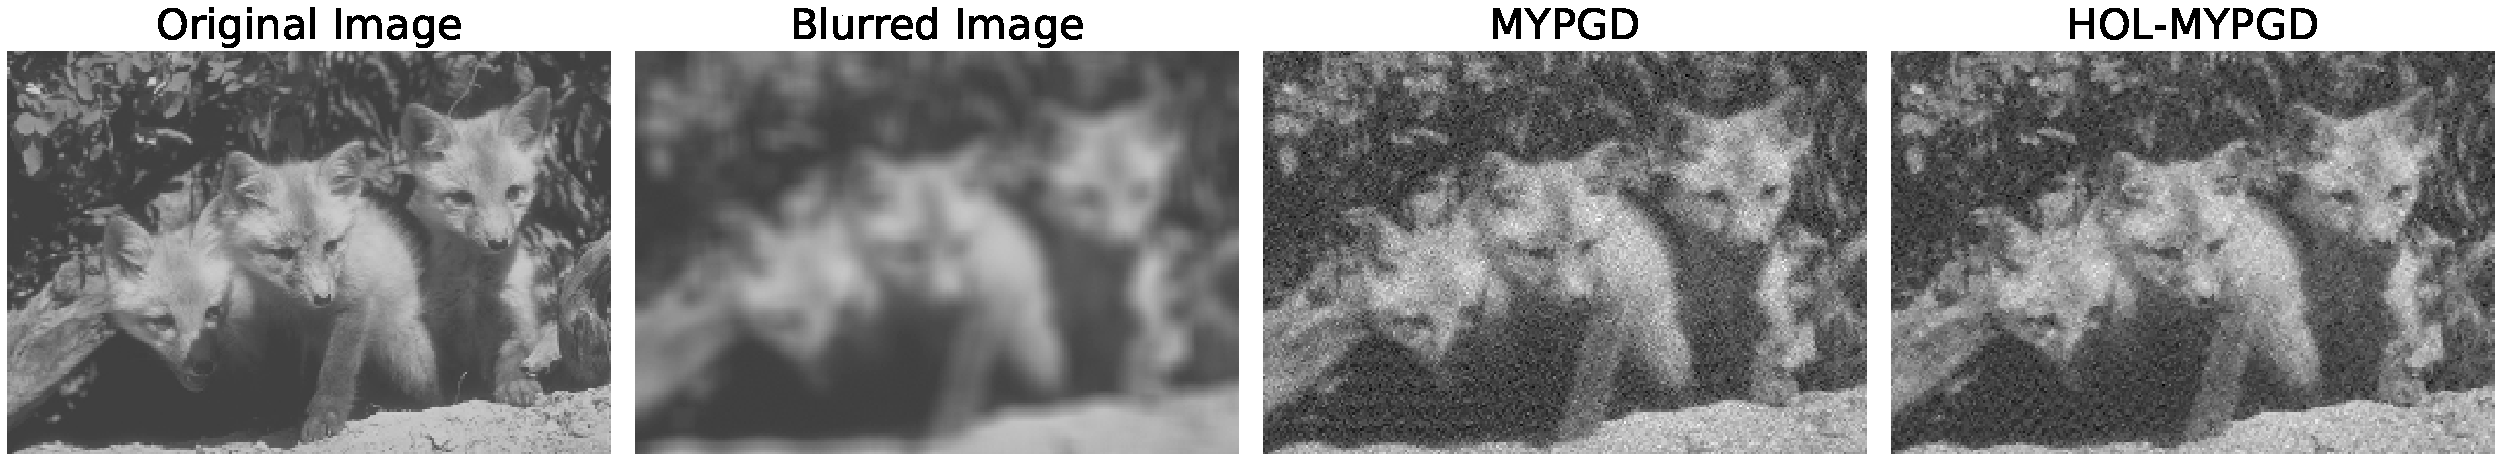
\includegraphics[width=\textwidth]{images/mmle/mmle_deblurring_image_appendix1.pdf}
    \caption{Setup B deblurring image comparison 1.}
    \label{fig:setup_e_images1}
\end{figure}

\begin{figure}[htbp]
    \centering
    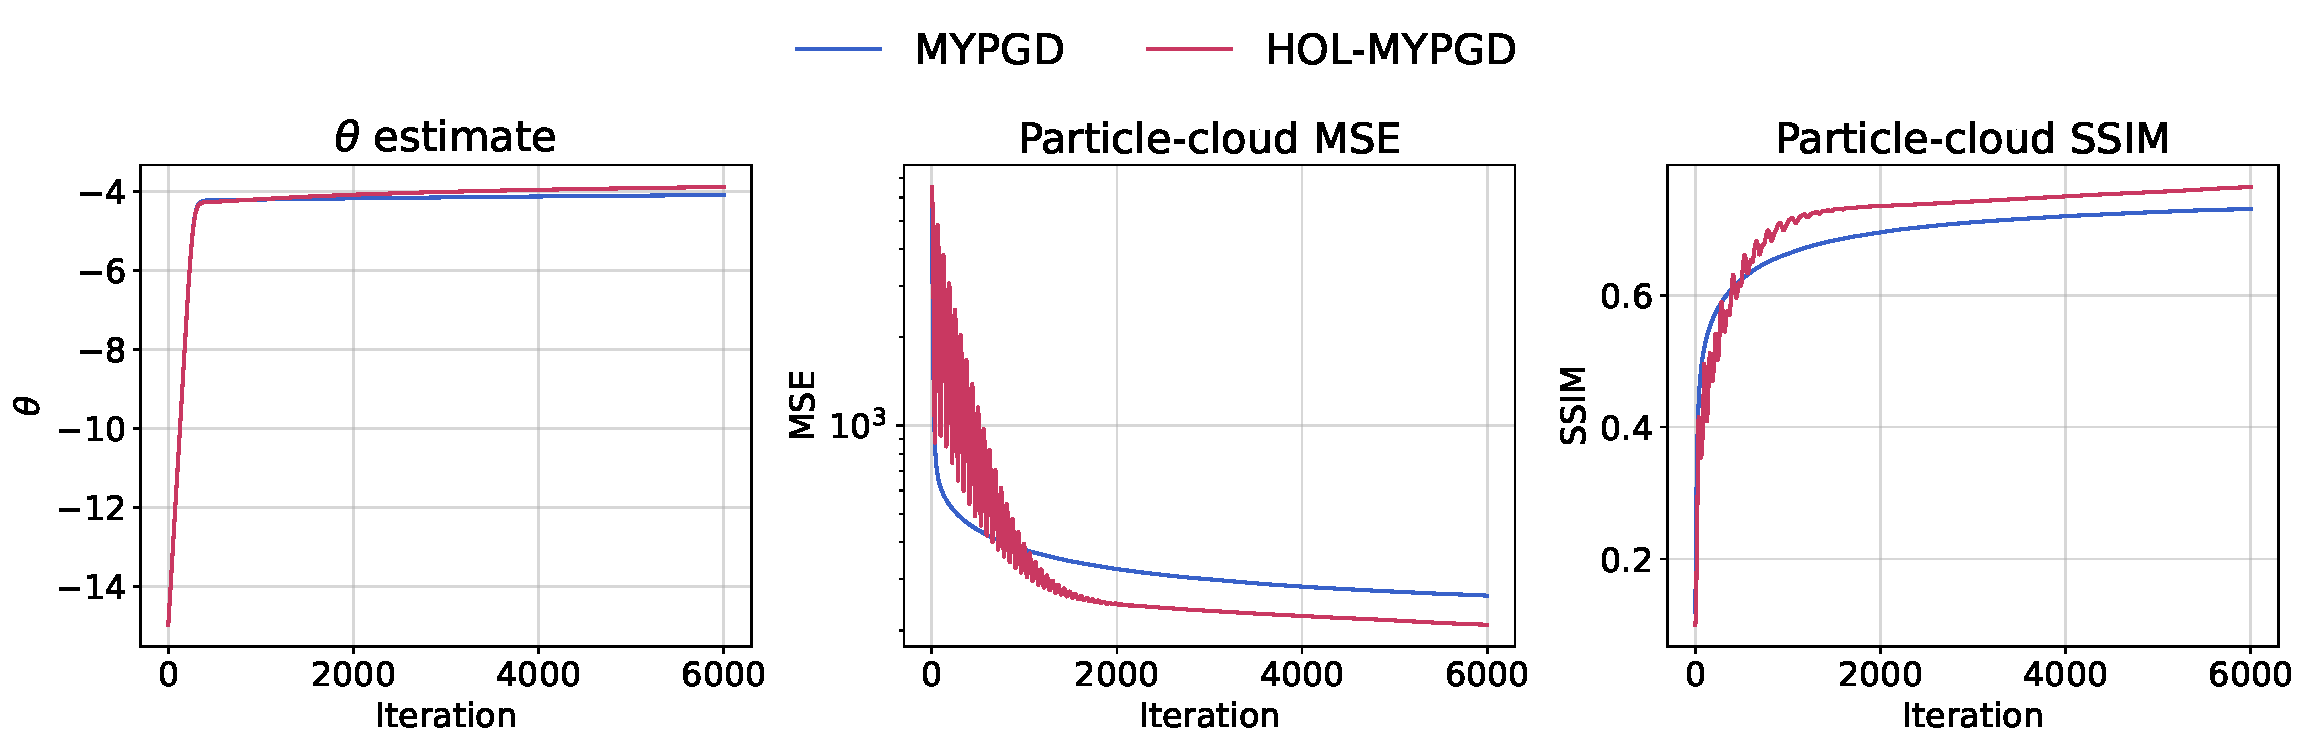
\includegraphics[width=\textwidth]{images/mmle/mmle_deblurring_graphs_appendix1.pdf}
    \caption{Setup B deblurring convergence comparison 1.}
    \label{fig:setup_e_graphs1}
\end{figure}

\begin{figure}[htbp]
    \centering
    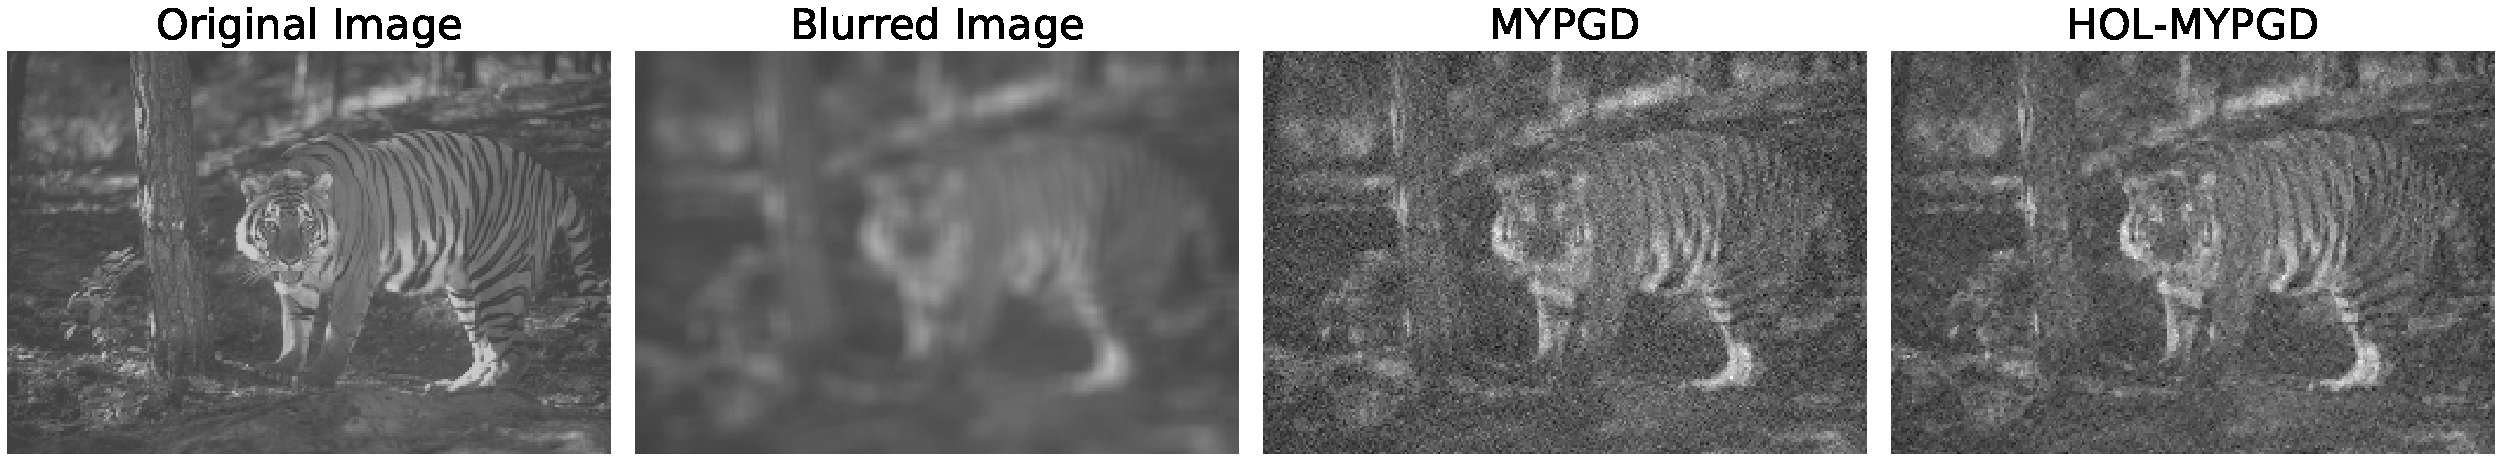
\includegraphics[width=\textwidth]{images/mmle/mmle_deblurring_image_appendix2.pdf}
    \caption{Setup B deblurring image comparison 2.}
    \label{fig:setup_e_images2}
\end{figure}

\begin{figure}[htbp]
    \centering
    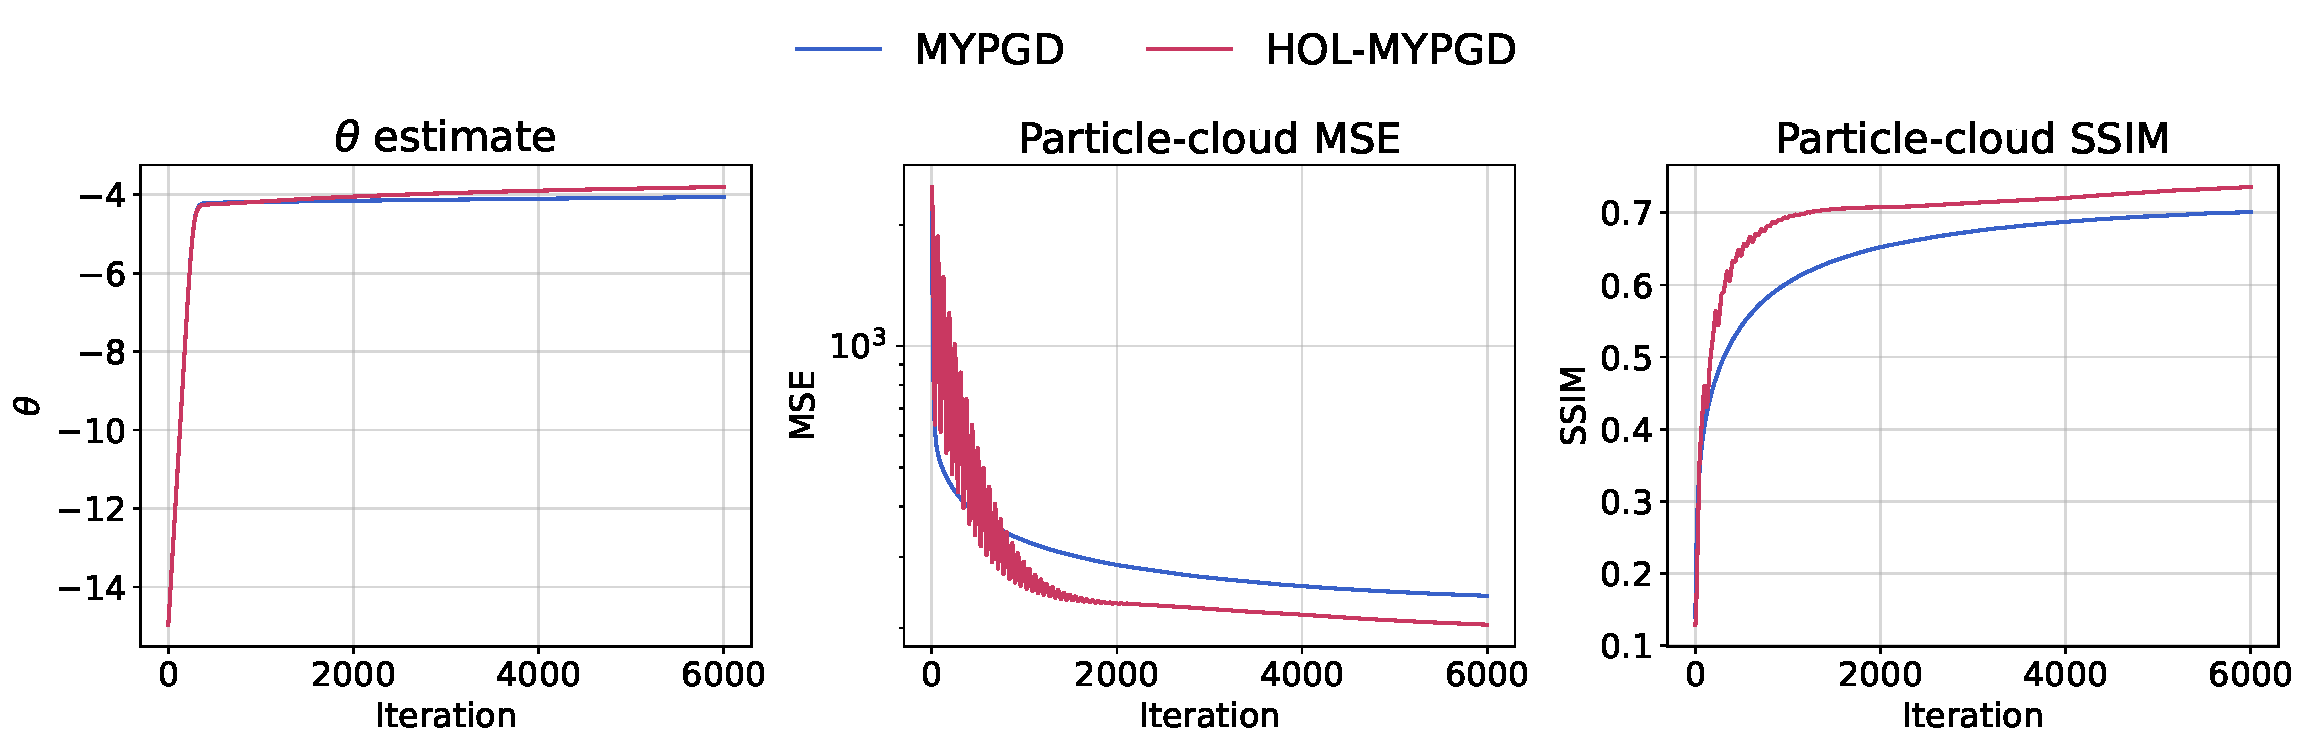
\includegraphics[width=\textwidth]{images/mmle/mmle_deblurring_graphs_appendix2.pdf}
    \caption{Setup B deblurring convergence comparison 2.}
    \label{fig:setup_e_graphs2}
\end{figure}

\begin{figure}[htbp]
    \centering
    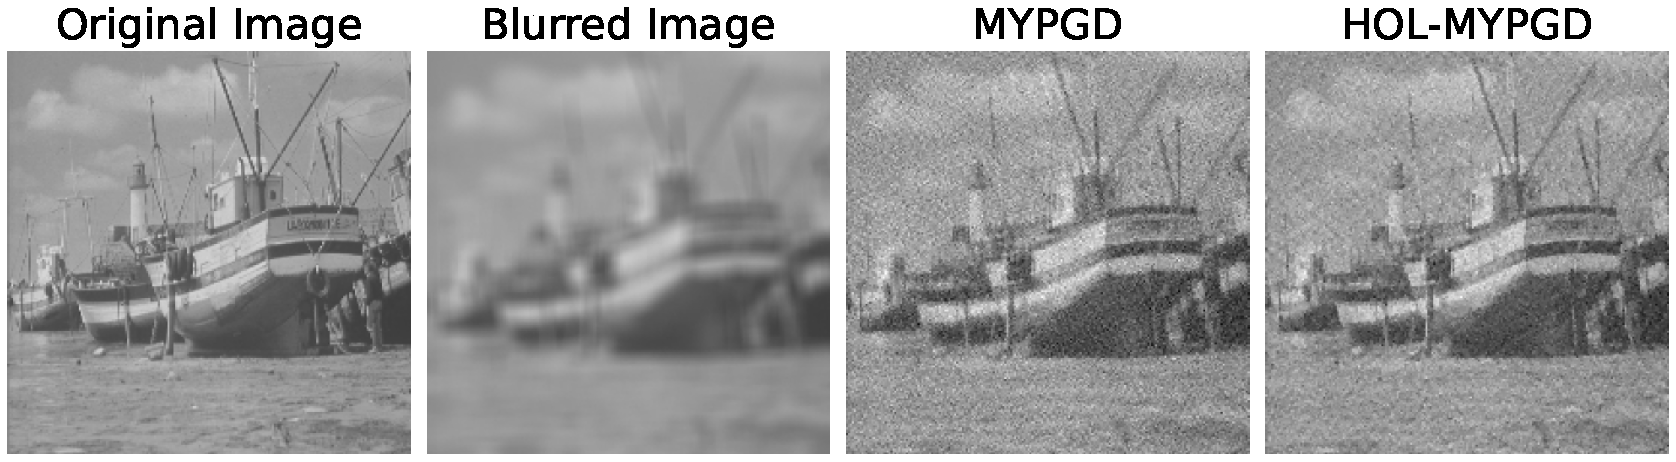
\includegraphics[width=\textwidth]{images/mmle/mmle_deblurring_image_appendix3.pdf}
    \caption{Setup B deblurring image comparison 3.}
    \label{fig:setup_e_images3}
\end{figure}

\begin{figure}[htbp]
    \centering
    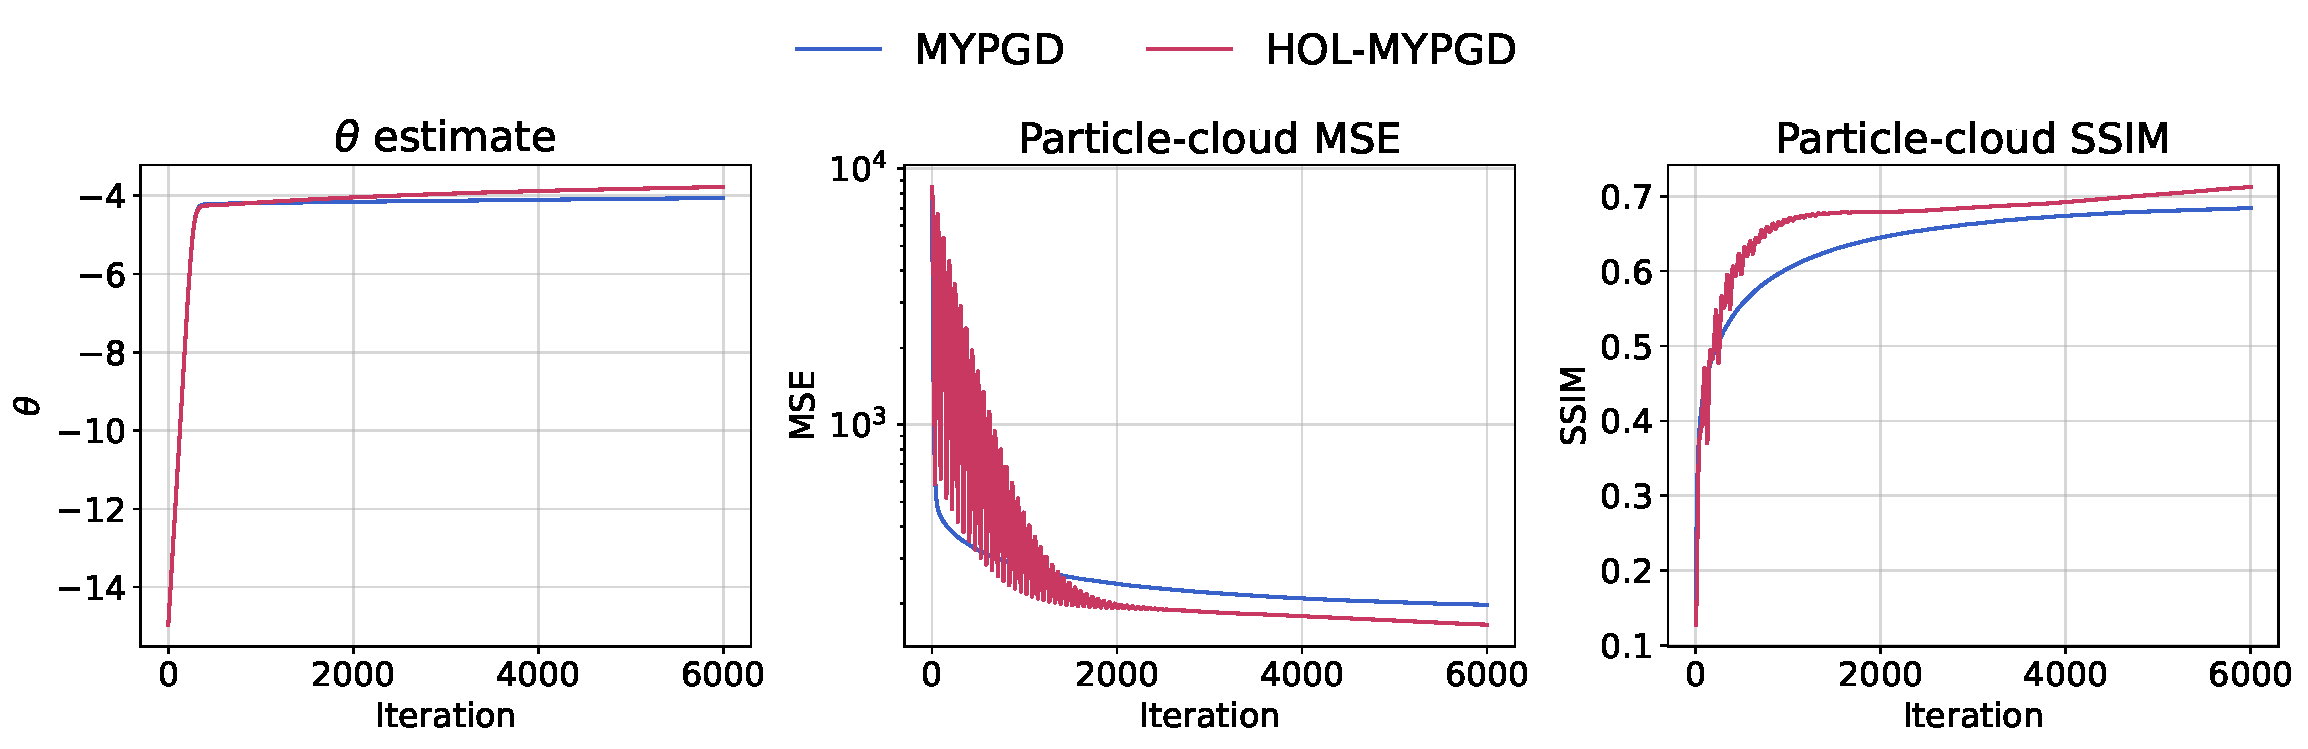
\includegraphics[width=\textwidth]{images/mmle/mmle_deblurring_graphs_appendix3.pdf}
    \caption{Setup B deblurring convergence comparison 3.}
    \label{fig:setup_e_graphs3}
\end{figure}